% ┌────────────────────────────────────────────────────────────────────────────┐
% │ ANGIO PAPER                                                                │
% │   Endoscopic hemostasis makes the difference: Angiographic treatment in    │
% │   patients with lower gastrointestinal bleeding                            │
% └────────────────────────────────────────────────────────────────────────────┘

\chapter{Angiography for Gastrointestinal Bleeding}
\sectionmark{Angiography for Gastrointestinal Bleeding}

This retrospective study's goal was the identification of variables that
increase the chance for a patient suffering from lower gastrointestinal
bleeding (LGIB) to benefit from angiography.

LGIB describes any form of gastrointestinal (GI) bleeding occurring in the
lower gastrointestinal tract, which includes most of the small intestine and
all of the large intestine \citep{Treuting2018}. GI bleeding can have many
causes, including cancer, and the resulting blood loss can lead to shock,
syncope, and even death with a chance of around \SI{15}{\percent} in general
\citep{Rockey2005,PrasadKerlin2013,Wang2013,Kim2014}. While the majority of GI
bleedings subside on their own or can be arrested through endoscopic
treatment, endoscopy cannot detect the cause of LGIB in \SI{40}{\percent} of
all cases \citep{Yamada2015,Werner2018}. Once localised, though, over
\SI{90}{\percent} of LGIBs can be treated successfully. It is therefore vital
that in cases with symptoms severe enough to result in hospitalisation, the
source of bleeding is identified quickly and reliably and that hemostasis is
achieved, be that through endoscopic treatment or surgery \citep{Strate2010,
Werner2018}.

It is at this point that angiography comes into the picture. Angiography is a
medical radiological imaging technique that visualises blood vessels, as well
as bleeding. This is achieved by injecting a radio-opaque contrast agent into
the bloodstream in conjunction with X-ray imaging \citep{Martin2015}. Catheter
angiography (CA), coupled with transarterial embolisation (TAE), a method to
stop the flow of blood to a selected area of tissue, has high technical
success rates of \SIrange{90}{100}{\percent} and low complication rates of
\SIrange{1}{5}{\percent} \citep{Tan2008,Evangelista2000,Strate2010,Kim2017,
Lee2018,Oakland2019,Pannatier2019}. However, it also exposes the patient to
the  contrast agent and X-ray imaging, while endoscopy requires only
anaesthesia. Angiography is also a more complex technique and involves the
patient's referral to a radiologist. Thus, the decision of when to conclude
endoscopic procedures and begin angiographic treatment is challenging. If
angiography is initiated too late, the patient is subjected to multiple
failed endoscopies, while if angiography is used too early, the patient is
needlessly exposed to the side effects of radiological and surgical treatment.

Accordingly, our goal was to construct a decision-making aid for clinicians,
assisting them in deciding when to apply endoscopy and when to apply
angiography to treat LGIB. While prospective investigations will be required
to consolidate our results, the predictors we selected may contribute to the
development of future official guidelines.

\subsubsection{Methodology}\label{subsubsec:angiomethod}
\addcontentsline{toc}{subsection}{Methodology}
The data for this study was collected over the span of \num{11} years at a
maximum care hospital and included \num{133} patients. Of these, the treatment
group consisted of \num{41} patients that received CA for LGIB, while the
control group of \num{92} patients was treated for LGIB without angiography.
\num{110} variables were recorded for each patient, of which \num{20} were
designated as being of particular clinical relevance according to expert
opinion.

As the data collection period was so extensive and involved many clinicians,
no precise statements concerning the methods used for data recording can be
made. The data types were also highly diverse, ranging from binary labels,
such as clinical success, time intervals and ordinal variables, to numeric
laboratory test results.

\subsubsection{Analysis}\label{subsubsec:angioanalysis}
\addcontentsline{toc}{subsection}{Analysis}
All of our data was ultimately recorded by humans and was thus flawed, which
may sound harsh but is true more often than not. For example,
\citet{Gotzsche1989} reports that \SI{76}{\percent} of the \num{196} analysed
drug trials to treat rheumatoid arthritis contained \enquote{doubtful or
invalid statements} \citep{Brown2018}. Therefore, data cleaning and validation
was the first step, an arduous step that is nonetheless crucial.

Descriptive statistics followed, along with na\"{i}ve pairwise correlation
analyses between selected variables and nonparametric tests, using either
Fisher's exact test or the Mann-Whitney U test, depending on the data at hand
\citep{Winters2010} (see also \nameref{sec:methoverview}).

At the start of the principal analysis, two items had to be considered .
Firstly, we had to establish that we assume the professional decision of the
clinicians to treat a patient either with or without angiography to be founded
in their medical expertise. The alternative assumption would be that we cannot
equate a patient receiving angiographic treatment with the need of a patient
to receive such treatment. Under this alternative assumption, our
investigation could not have drawn any meaningful conclusions. It is a natural
limitation of a retrospective study, which is also why prospective
investigations are necessary before an official guideline can be established.
Hence, we assume that a causal link exists between a patient's statistics and
treatment.

\begin{figure}[b!]
\centering
 \makebox[\textwidth][l]{
   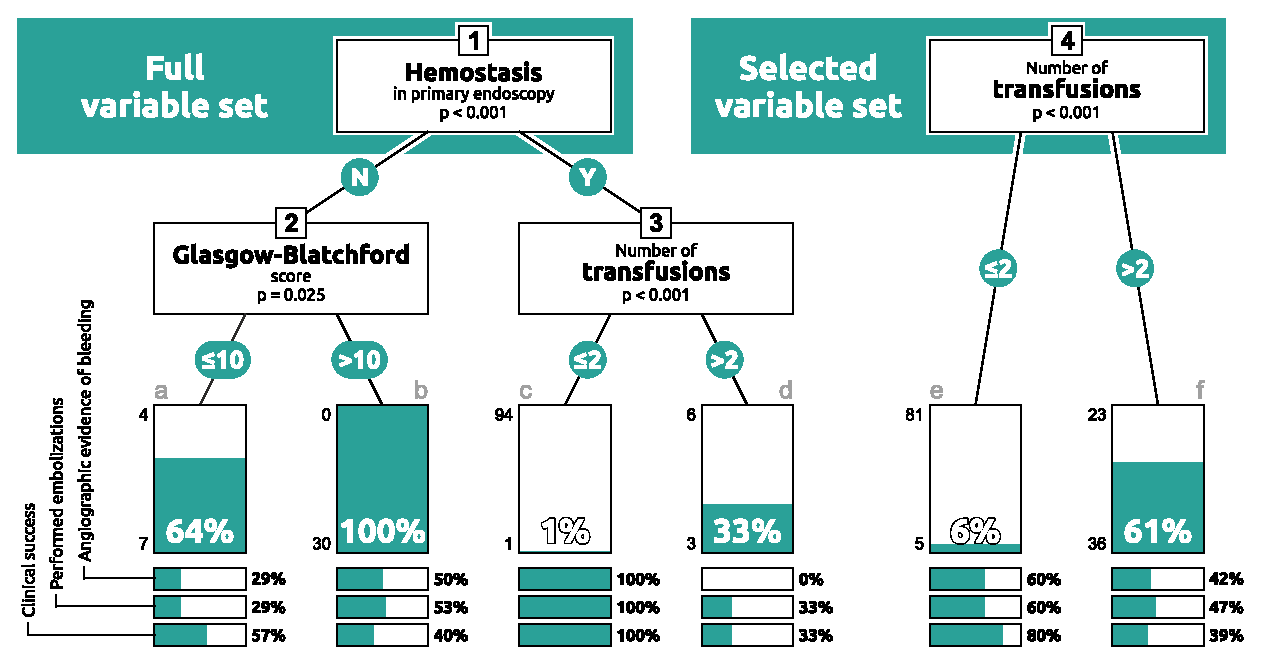
\includegraphics[width=\textwidth+\marginparwidth+\marginparsep]{
     04_GraphicFiles/03_angio_trees.eps}}
\caption{Modification of figures 2 and 3 from \citet{Werner2021}. Conditional
  inference trees were constructed from either the complete data set (left) or 
  a set of variables selected for clinical relevance (right). Each binary 
  split (numbered boxes 1 to 4) is annotated with its p-value. Each terminal 
  node (vertical bars a to f) shows the percentage of angiography-positive 
  cases.}
\label{fig:angiotree}
\end{figure}

Secondly, our goal was to create a decision-making aid for clinicians, helping
them decide when to switch from endoscopy to angiography for the treatment of
LGIB. While we could have constructed a complex regression model to predict
the method suitable for a patient as best as possible, such a model would not
be applicable in the daily clinic routine. While computer-based predictors to
guide treatment decisions may become mundane in the future, this is not yet
the case. Consequently, our decision-making aid needed to be easily traceable,
allowing the clinician to arrive at a prognosis by following a transparent
algorithm. Accepting that, in consequence, our final model may be undercomplex
to some extent and thus prone to underfitting, we elected to use conditional
inference trees (see \nameref{sec:methoverview}).

\begin{figure}[b!]
\centering
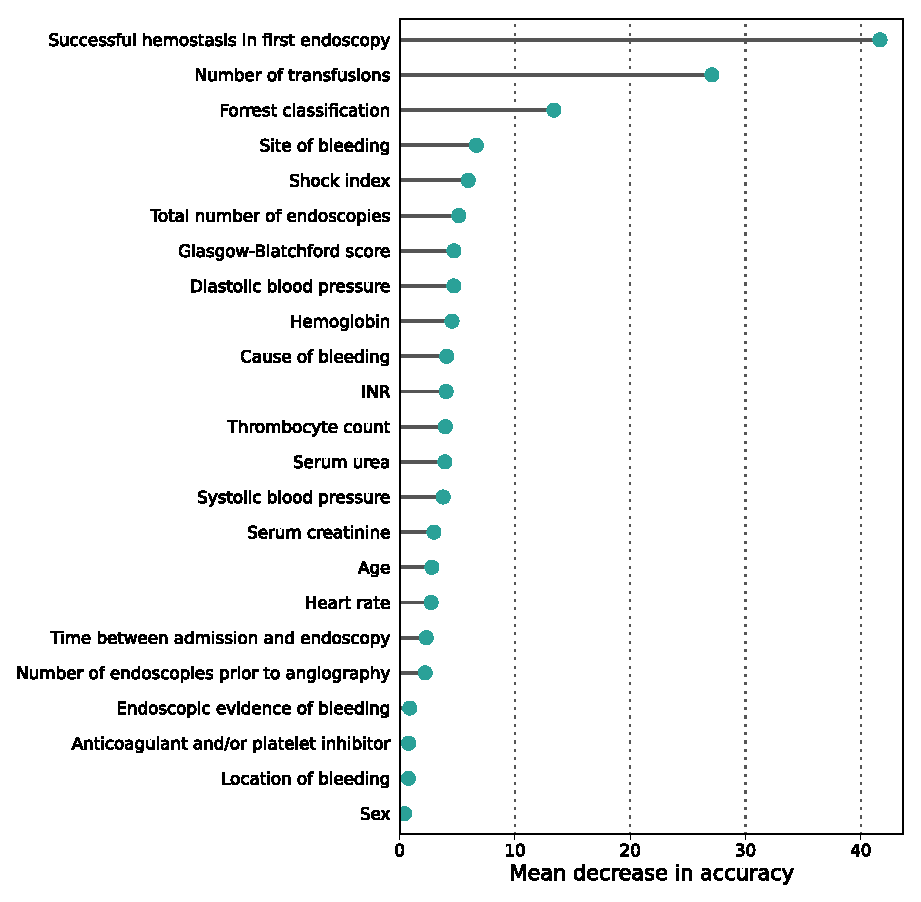
\includegraphics[width=\textwidth]{04_GraphicFiles/03_angio_forest.eps}
\caption{Modification of figure 1 from \citet{Werner2021}. Variable importance
  in terms of mean decrease in accuracy of the features included in the   
  construction of the decision trees computed using a random forest
  classifier with \num{10000} trees and \num{25} iterations.}
\label{fig:angioforest}
\end{figure}

We decided to construct two decision trees shown in \cref{fig:angiotree}, one
based on all recorded patient variables and another based solely on the
clinically relevant variables. The trees offer a straightforward way for a
clinician to determine if a patient should receive angiography or not. Using
the tree based on the full variable set as an example, only two queries are
needed for a patient: If hemostasis was achieved in the first endoscopy, the
number of blood transfusions a patient has received is needed as input. On the
other hand, if the primary endoscopy failed to achieve hemostasis, the Glasgow-
Blatchford Bleeding Score (GBS) of the patient becomes the telling factor. The
GBS is used to classify the severity of GI bleeding \citep{Laursen2015}.
\pagebreak

% page break ...................................................................

\noindent
In addition, we also used random forest to compute the mean decrease in
accuracy variable importance measure for the variables used in constructing
the decision trees \citep{Han2016} (see also \nameref{sec:methoverview}). This
was done to substantiate the variable choices made by the decision tree
models. Mean decrease in accuracy is computed by permuting the out-of-bag (OOB)
data, referring to the data not included in an individual bootstrap sample.
The error rate on the OOB data is computed once and computed again after
permuting each predictor variable.  The difference between the two is averaged
over all bootstrap samples and normalised by the standard deviation of the
differences. The resulting variable importance is a positive value that
increases the more influential any given variable is. The results agreed
satisfactorily with the decision trees, with the success of achieving
hemostasis in the primary endoscopy (binary split 1 in \cref{fig:angiotree})
and the number of transfusions (binary splits 3 and 4 in \cref{fig:angiotree})
being the two most important variables.

\vfill
\noindent My contribution to this publication was the complete bioinformatic
and statistical analysis.\nopagebreak
\medskip
\begin{tcolorbox}[
  boxrule=0pt, leftrule=1pt, colframe=s-blue, colback=white, sharp corners=all]%
  \raggedright
  Werner, DJ., Baar, T., Kiesslich, R., Wenzel, N., Abusalim, N., Tresch, A.,
  Rey, JW. (2021).
  
  \smallskip
  \href{https://www.wjgnet.com/1948-5190/full/v13/i7/221.htm}
    {Endoscopic hemostasis makes the difference: Angiographic treatment in
    patients with lower gastrointestinal bleeding}

  \smallskip
  \textit{World J Gastrointest Endosc, 13(7): 221-232}
\end{tcolorbox}

% ┌────────────────────────────────────────────────────────────────────────────┐
% │ PDF                                                                        │
% └────────────────────────────────────────────────────────────────────────────┘

\includepdf[pages={4-15}, addtotoc={4, section, 1,
  Endoscopic hemostasis makes the difference: Angiographic treatment in
  patients with lower gastrointestinal bleeding,
  Endoscopic hemostasis makes the difference: Angiographic treatment in
  patients with lower gastrointestinal bleeding}]
  {"07_Publications/Werner2021.pdf"}

\null
\thispagestyle{empty}
\newpage